\documentclass{article}
\usepackage[margin=1.5cm]{geometry} %Feel free to adjust this margin to your liking
\usepackage[utf8]{inputenc} %So we can use special characters
\usepackage{graphicx} %You might need this to include an image
\usepackage{amsmath} %For various math functions..
\usepackage{hyperref} %For creating hyperlinks

%opening
\title{Database assignment 2}
\author{Daniel Lin and Robert Arntzenius}

\begin{document}

\maketitle

\section{Relational Algebra}

\subparagraph*{Exercize 1}
-

\chapter{1.}


\pi_{\text{mid}}
\sigma_{\text{"title" = "Not clickbait"} \wedge \text{"likecount"} > 9000 }messages


\chapter{2.}


\rho(invited, \pi_{\text{id}}((\pi_{\text{eid}} \sigma_{\text{name="Cheap sunglasses check description"}} event)\bowtie_{{eid}} 
invitedToEvent))\bowtie_{\text{id}} user)

\rho(users, \pi_{\text{id}}user)

\pi_{\text{id}}(invited \bowtie_{\text{invited.id $ \neq $ user.id}} users)

\chapter{3.}

\rho(mes1, message)

\rho(mes2, message)

\rho(res, \pi_{\text{mes1.mid}} ( (message \times message) - \sigma_{\text{mes1.likecount} < \text{mes2.likecount}}(mes1 \times mes2) ) )

\pi_{\text{id}}(\pi_{\text{mid}}(res)\bowtie_{\text{mid}}messageLikes)\bowtie_{\text{id}}user

\chapter{4.}

\rho(invited, \pi_{\text{id}}(\sigma_{\text{accepted = "true"}}(\pi_{\text{eid}} \sigma_{\text{name="Nude painting"}} event)\bowtie_{{eid}} 
invitedToEvent))\bowtie_{\text{id}} user)

\rho(users, \pi_{\text{id}}user)

%grab friends
\rho(friends, \pi_{\text{id}}(\pi_{fid}friend)\bowtie_{id}user)


\pi_{\text{name}}(invited \bowtie_{\text{invited.id = user.id}} users \cup friends)



\chapter{5.}

\rho(friends, \pi_{\text{id}}(\pi_{fid}friend)\bowtie_{id}user)

\rho(othergender, \pi_{\text{id}}friends - \pi_{\text{id}}(\pi_{\text{id}}friends)\bowtie_{\text{gender}} user)

%this might not work yet
\rho(otherage, \pi_{\text{id}}(\pi_{\text{id}}friends)\bowtie_{\text{friends.age} < \text{user.age}}user)

\pi_{\text{name}}(friends/(othergender \cap otherage))user


\chapter{6.}

\rho(one, \pi_{\text{id}}\sigma_{\text{name = "Crazy Cosplay Caroline"}}user)

\rho(onemessages, \pi_{\text{mid}}\rho_{\text{creator=one}}message)

%grab people that have liked the message
\rho(messageliked, \pi_{\text{id}}\sigma_{\text{mid=onemessages}}messageLikes)

%give names
\pi_{\text{name}}((messageliked)/(\pi_{\text{id, name}}user))


\chapter{7.}


%tip was to use cartesian product
%or self-joins
\rho(mes1, \sigma_{likecount > 999}message)

\rho(mes2, \sigma_{likecount > 999}message)

\rho(mes3, \sigma_{likecount > 999}message)

\rho(res1, \pi_{\text{mes1.creator}} (\sigma_{\text{mes1.mid} \neq \text{mes2.mid} \wedge \text{mes2.mid} \neq \text{mes3.mid} \wedge \text{mes1.mid}  \neq \text{mes3.mid}}(mes1 \times mes2 \times mes3) ) )

\rho(res2, \pi_{\text{mes2.creator}} (\sigma_{\text{mes1.mid} \neq \text{mes2.mid} \wedge \text{mes2.mid} \neq \text{mes3.mid} \wedge \text{mes1.mid}  \neq \text{mes3.mid}}(mes1 \times mes2 \times mes3) ) )

\rho(res3, \pi_{\text{mes3.creator}} (\sigma_{\text{mes1.mid} \neq \text{mes2.mid} \wedge \text{mes2.mid} \neq \text{mes3.mid} \wedge \text{mes1.mid}  \neq \text{mes3.mid}}(mes1 \times mes2 \times mes3) ) )


\pi_{\text{id}}(\sigma_{\text{res1.creator} = \text{res2.creator} \wedge \text{res2.creator} = \text{res3.creator} \wedge \text{res1.creator}  = \text{res3.creator}}(res1 \times res2 \times res3)})\bowtie_{res.creator=user.id}user

\section{Shema Normalization}

\subparagraph*{Exercize 2}
-

\chapter{1.}

Determine all the functional dependencies (F) that are derivable from the points mentioned above.

	V \rightarrow TUCSD	(\text{A video ID implies all video attributes})
	
  UT \rightarrow V	(\text{Since an uploader cannot upload more than one video with the same title,}
  
  these attributes implie the video ID)

  S \rightarrow C	(\text{Since subcategories are unique per category, there are no subcategories placed in more than one}
  
  \text{ category})

	N \rightarrow BA		(\text{Since a comment number is unique, it implies all comment attributes})
	
  N \rightarrow U	(\text{Since a comment number is unique and used by the same account used for uploading, it implies the}
  
  uploader)

  N \rightarrow V		(\text{Since every comment is linked via its number to a single video ID, the comment number implies the}
  
  video ID)
\\


\chapter{2.}
Determine the key(s) in this table

\newline


	N \rightarrow V, V \rightarrow TUCSD 
	
	implies N \rightarrow TUCSD					(Transitivity)
	
\newline
	
	N \rightarrow BA, N \rightarrow U, N \rightarrow V, N \rightarrow TUCSD 
	
	implies N \rightarrow BAUVTUCSD		(Union)
\newline
	
Since N is never on the right side, 

N is certainly part of all existing keys and since N is a key of itself,

N must be the only existing key.

\newline

\chapter{3.} Derive a minimal cover (G) for R

First, we listed all FD's:

	V \rightarrow T
	
	V \rightarrow U
	
	V \rightarrow C
	
	V \rightarrow S
	
	V \rightarrow D
	
	UT \rightarrow V
	
	S \rightarrow C
	
	N \rightarrow A
	
	N \rightarrow B
	
	N \rightarrow U
	
	N \rightarrow V

	Then we try to derive existing FD's from others:
	
	N → V, V → U implies N → U						(Transitivity)
	
	So, we delete N → U from the list
	
	\\
\newline

	Finally, we write down the minimal cover:
	V \rightarrow TUCSD
	UT \rightarrow V
	S \rightarrow C
	N \rightarrow ABV
	
	\newline	\break

\chapter{4.}

Using your minimal cover, derive a lossless join decomposition in BCNF and indicate a primary key for each table in the decomposition.
\newline

VTUCSDNBA

\Downarrow \> \Rightarrow NVBA

VTUCSD
	  
	The resulting lossless join decomposition in BCNF is: VTUCSD, NVBA

\chapter{5.}

Is your decomposition also dependency preserving? Why is or isn’t it? If it is not, derive a dependency preserving decomposition in 3NF.
\newline

The decomposition is not dependency preserving, because not all FD’s in the minimal cover have their own table


To make it dependency preserving, we add a table for all other FD’s, the resulting decomposition is:


VTUCSD, NVBA, UTV, SC

\chapter{6.}

Prove, if XY \rightarrow B and X \rightarrow Y then X \rightarrow B

	XY \rightarrow B
	
	X \rightarrow Y
	
	XX \rightarrow XY								(Augmentation X)
	
	XX \rightarrow B									(Transitivity XY → B)
	
	X \rightarrow B									(Union)	


\newline

\subparagraph*{Exercize 3}
-

\chapter{1.}

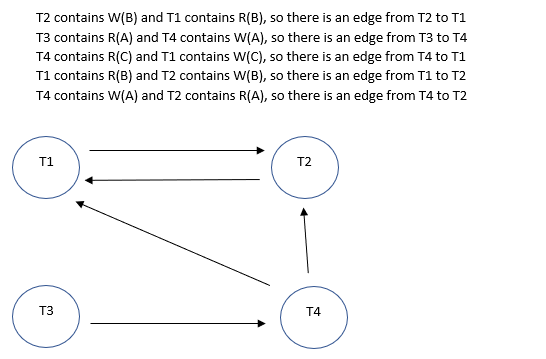
\includegraphics{./schema.png}

\chapter{2.}

The graph is not conflict serializable because there exists a cycle inbetween T1 and T2.

\chapter{3.}

{\small %you can try \tiny font size here for a smaller table
\begin{tabular}{|l||lllllllllllllll|}
\hline
T1:&R(C)& & & & &R(B)&W(C) &W(A)& & & & &&&Cmt.\\ \hline
T1:&S(C)& & & & &S(B)&X(C) &X(A)& & & & &&&Cmt.\\ \hline
T2:&& &R(B)& &W(B)& & & & & & &W(B) &R(A)& W(C)&Cmt.\\ \hline
T2:&& &S(B)& &X(B)& & & & & & &X(B) &S(A)& X(C)&Cmt.\\ \hline
T3:&&R(A)& &W(A) & & & & && &R(A) & & &&Cmt.\\ \hline
T3:&&S(A)& &X(A) & & & & && &S(A) & & &&Cmt.\\ \hline
T4:&& & & & & & & & R(C)& W(A)&& & &&Cmt.\\ \hline
T4:&& & & & & & & & S(C)& S(A)&& & &&Cmt.\\ \hline
\end{tabular}
}


\end{document}
